
\chapter{Configurazione Router}

\section{Overview della configurazione}

In questo capitolo andremo a connettere il router 4g alla rete vpn e aggiungere le opportune regole in modo che il traffico proveniente dall'host domotico sia indirizzato verso la VPN

\section{Creazione della configurazione OpenVPN}

Si devono seguire gli step descritti in sezione \ref{sec:client_keys}, quindi creare la certificate request e firmarla nel \it{server CA}. Per poi usare lo script creato in sezione \ref{sec:script_client} per costruire il file di configurazione:

\begin{bashcode}{Server}{}
$ ./make_config.sh router
\end{bashcode}


\section{Preparazione del Router 4g}

L'interfaccia grafica dovrebbe essere gia' installata e raggiungibile, in caso contrario puo' essere installata e configurata seguendo la guida ufficiale di \it{OpenWrt} \cite{install-luci}.

\begin{figure}[h]

    \centering

    \begin{subfigure}{0.5\textwidth}
        \centering
        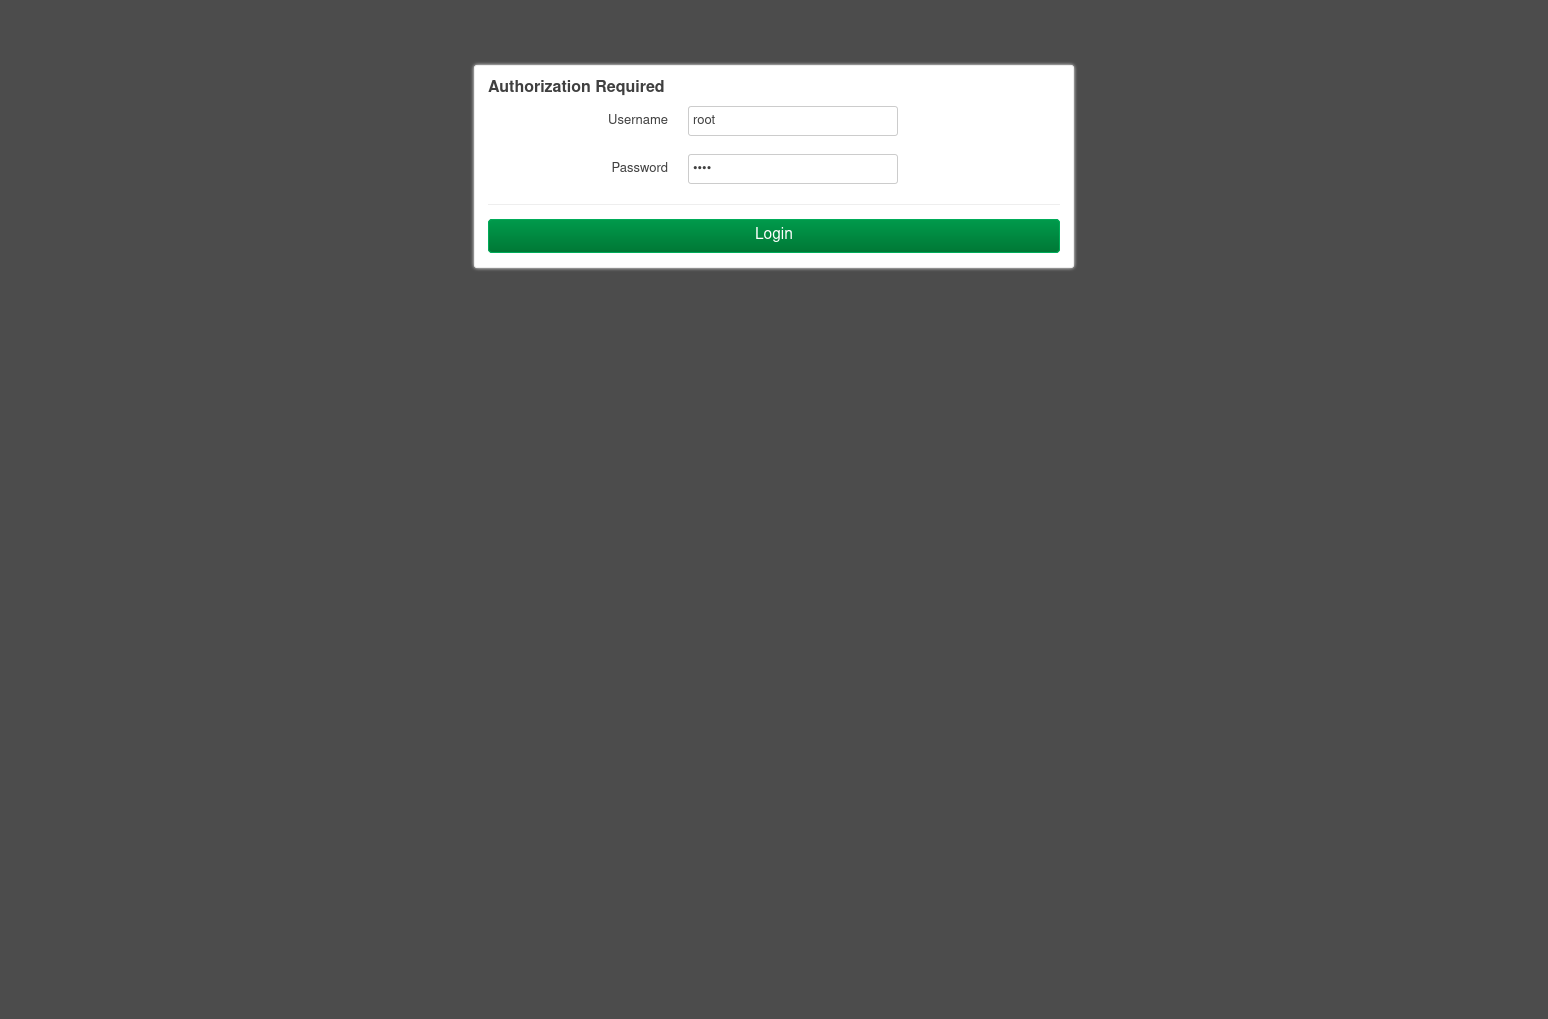
\includegraphics[height=0.6\linewidth]{immagini/LuCI_login}
        \caption{Login page}
        \label{fig:luci-login}
    \end{subfigure}%
    \hfill
    \begin{subfigure}{0.5\textwidth}
        \centering
        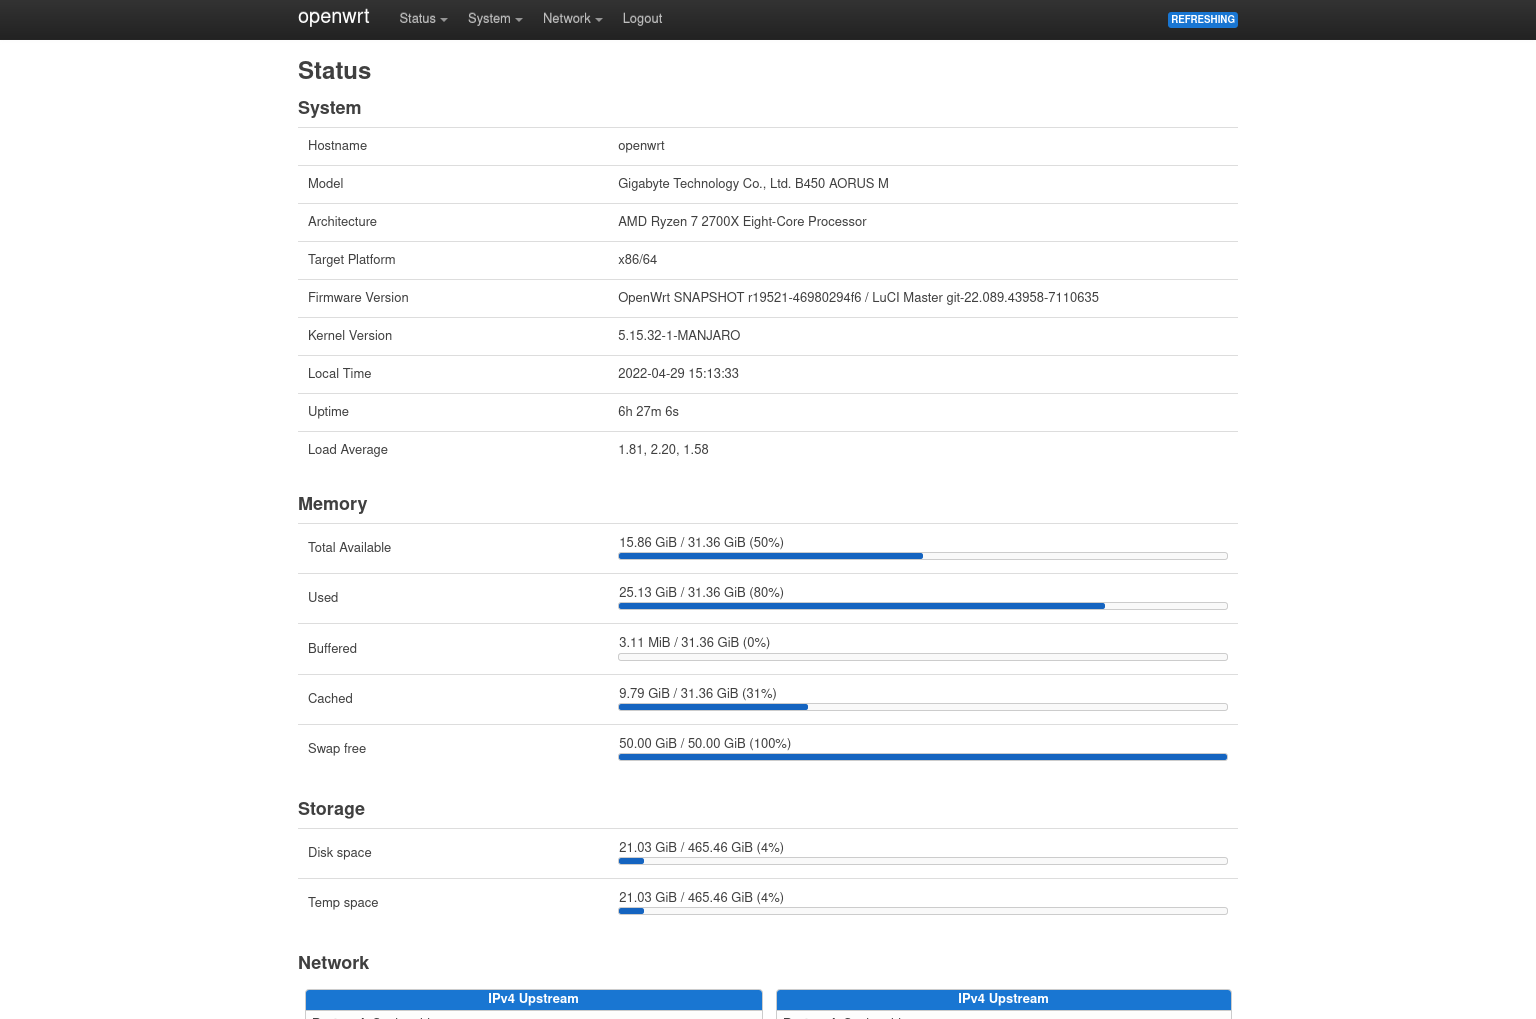
\includegraphics[height=0.6\linewidth]{immagini/LuCI_status}
        \caption{Status page}
        \label{fig:luci-status}
    \end{subfigure}%

    \begin{subfigure}{0.5\textwidth}
        \centering
        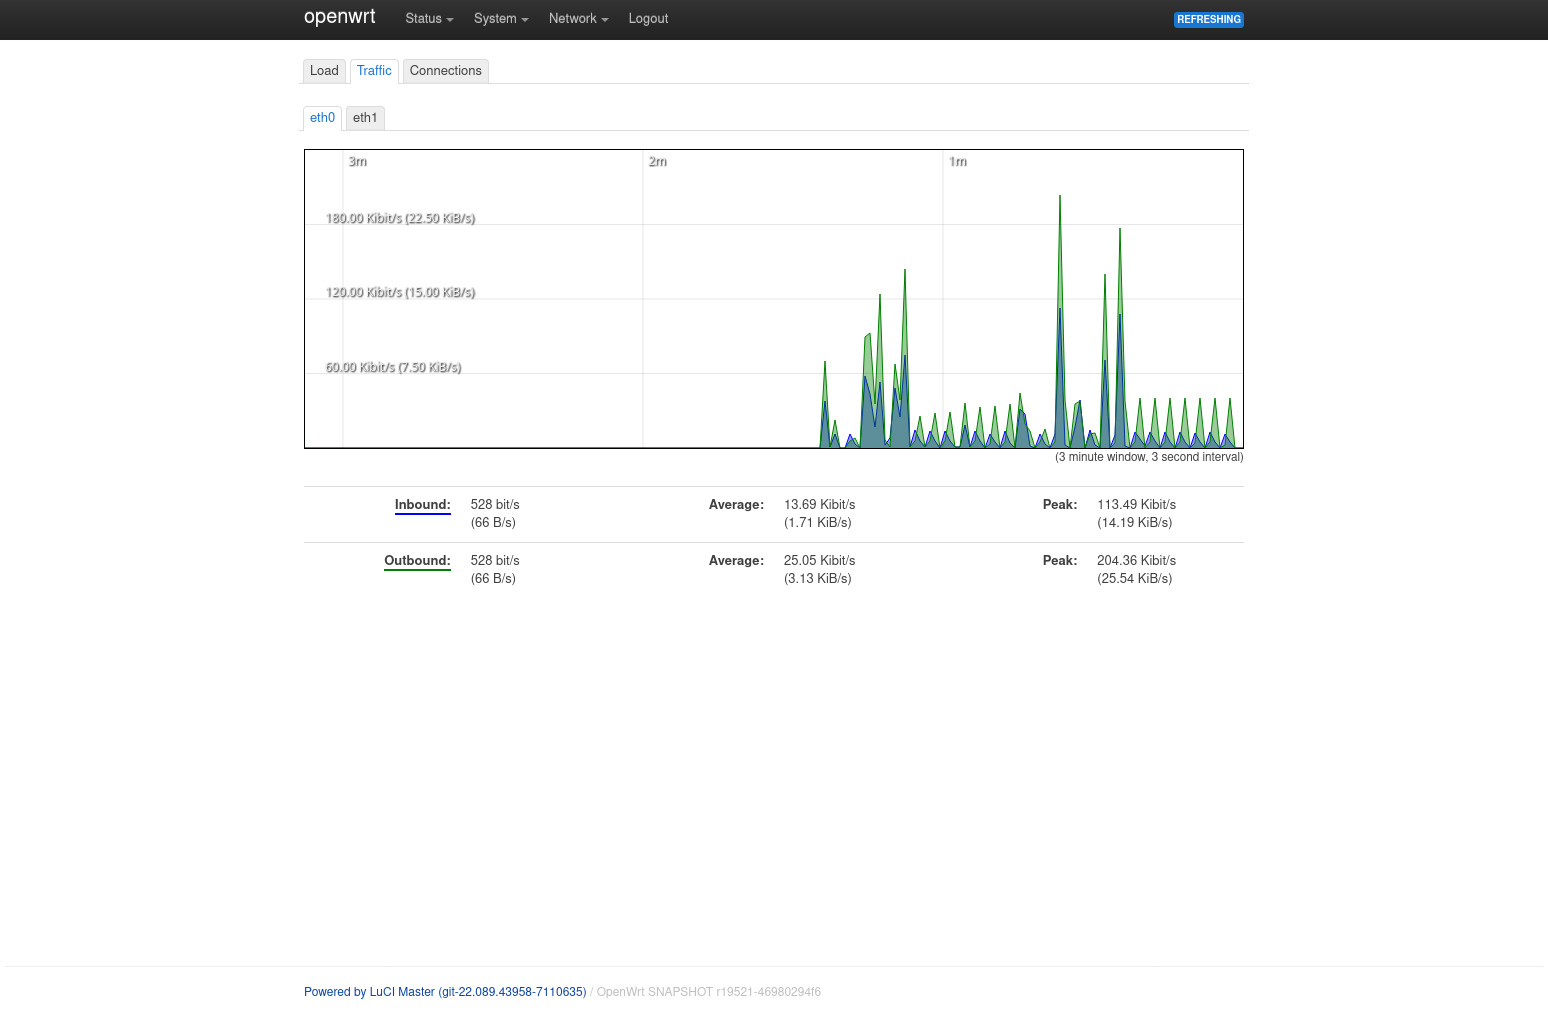
\includegraphics[height=0.6\linewidth]{immagini/LuCI_graphs}
        \caption{Graphs page}
        \label{fig:luci-graphs}
    \end{subfigure}%
    \caption{\#TODO caption}
\end{figure}


\begin{bashcode}{Router 4g}{}
BusyBox v1.35.0 (2022-04-24 21:09:51 UTC) built-in shell (ash)
    _______                     ________        __
    |       |.-----.-----.-----.|  |  |  |.----.|  |_
    |   -   ||  _  |  -__|     ||  |  |  ||   _||   _|
    |_______||   __|_____|__|__||________||__|  |____|
            |__| W I R E L E S S   F R E E D O M
    -----------------------------------------------------
    OpenWrt SNAPSHOT, r19521-46980294f6
    -----------------------------------------------------
\end{bashcode}
